% -*- TeX-engine: luatex -*-
\documentclass[aspectratio=169]{beamer}
\usepackage{luatexja}
\usepackage{luatexja-ruby}
\usepackage[hiragino-pro,deluxe]{luatexja-preset}
\usepackage{verbatim}
\usepackage[T1]{fontenc}
\usepackage{alltt}
\usepackage{graphicx}
\usepackage{xcolor}
\hypersetup{unicode}
\usepackage{fancyvrb}
\usepackage{amsmath}
\usepackage{ulem}
\usepackage{listings}
\usepackage{tikz}

\usetheme{CambridgeUS}
\renewcommand{\kanjifamilydefault}{\gtdefault}
\setbeamerfont{title}{family=\gtfamily} % ゴシック
\setbeamerfont{author}{family=\gtfamily} % ゴシック
\setbeamerfont{frame}{family=\gtfamily} % ゴシック
\setbeamerfont{frametitle}{family=\mgfamily} % 丸ゴシック
\setbeamertemplate{blocks}[rounded]

\title{区間演算と精度保証}
\author{荒田 実樹}
\date{2017年11月7日}

\newcommand{\hexa}[1]{[\texttt{#1}]_{16}}
\newcommand{\binary}[1]{[\texttt{#1}]_{2}}
\newcommand{\abs}[1]{\lvert #1\rvert}
\newcommand{\roundsto}{\stackrel{\text{丸め}}{\leadsto}}
\newcommand{\ub}[1]{\overline{#1}}
\newcommand{\lb}[1]{\underline{#1}}

\lstset{basicstyle=\ttfamily,columns=flexible,language=C}

\begin{document}
\begin{frame}[plain]\frametitle{宣伝}
  \centering
  \raisebox{-0.5\textheight}{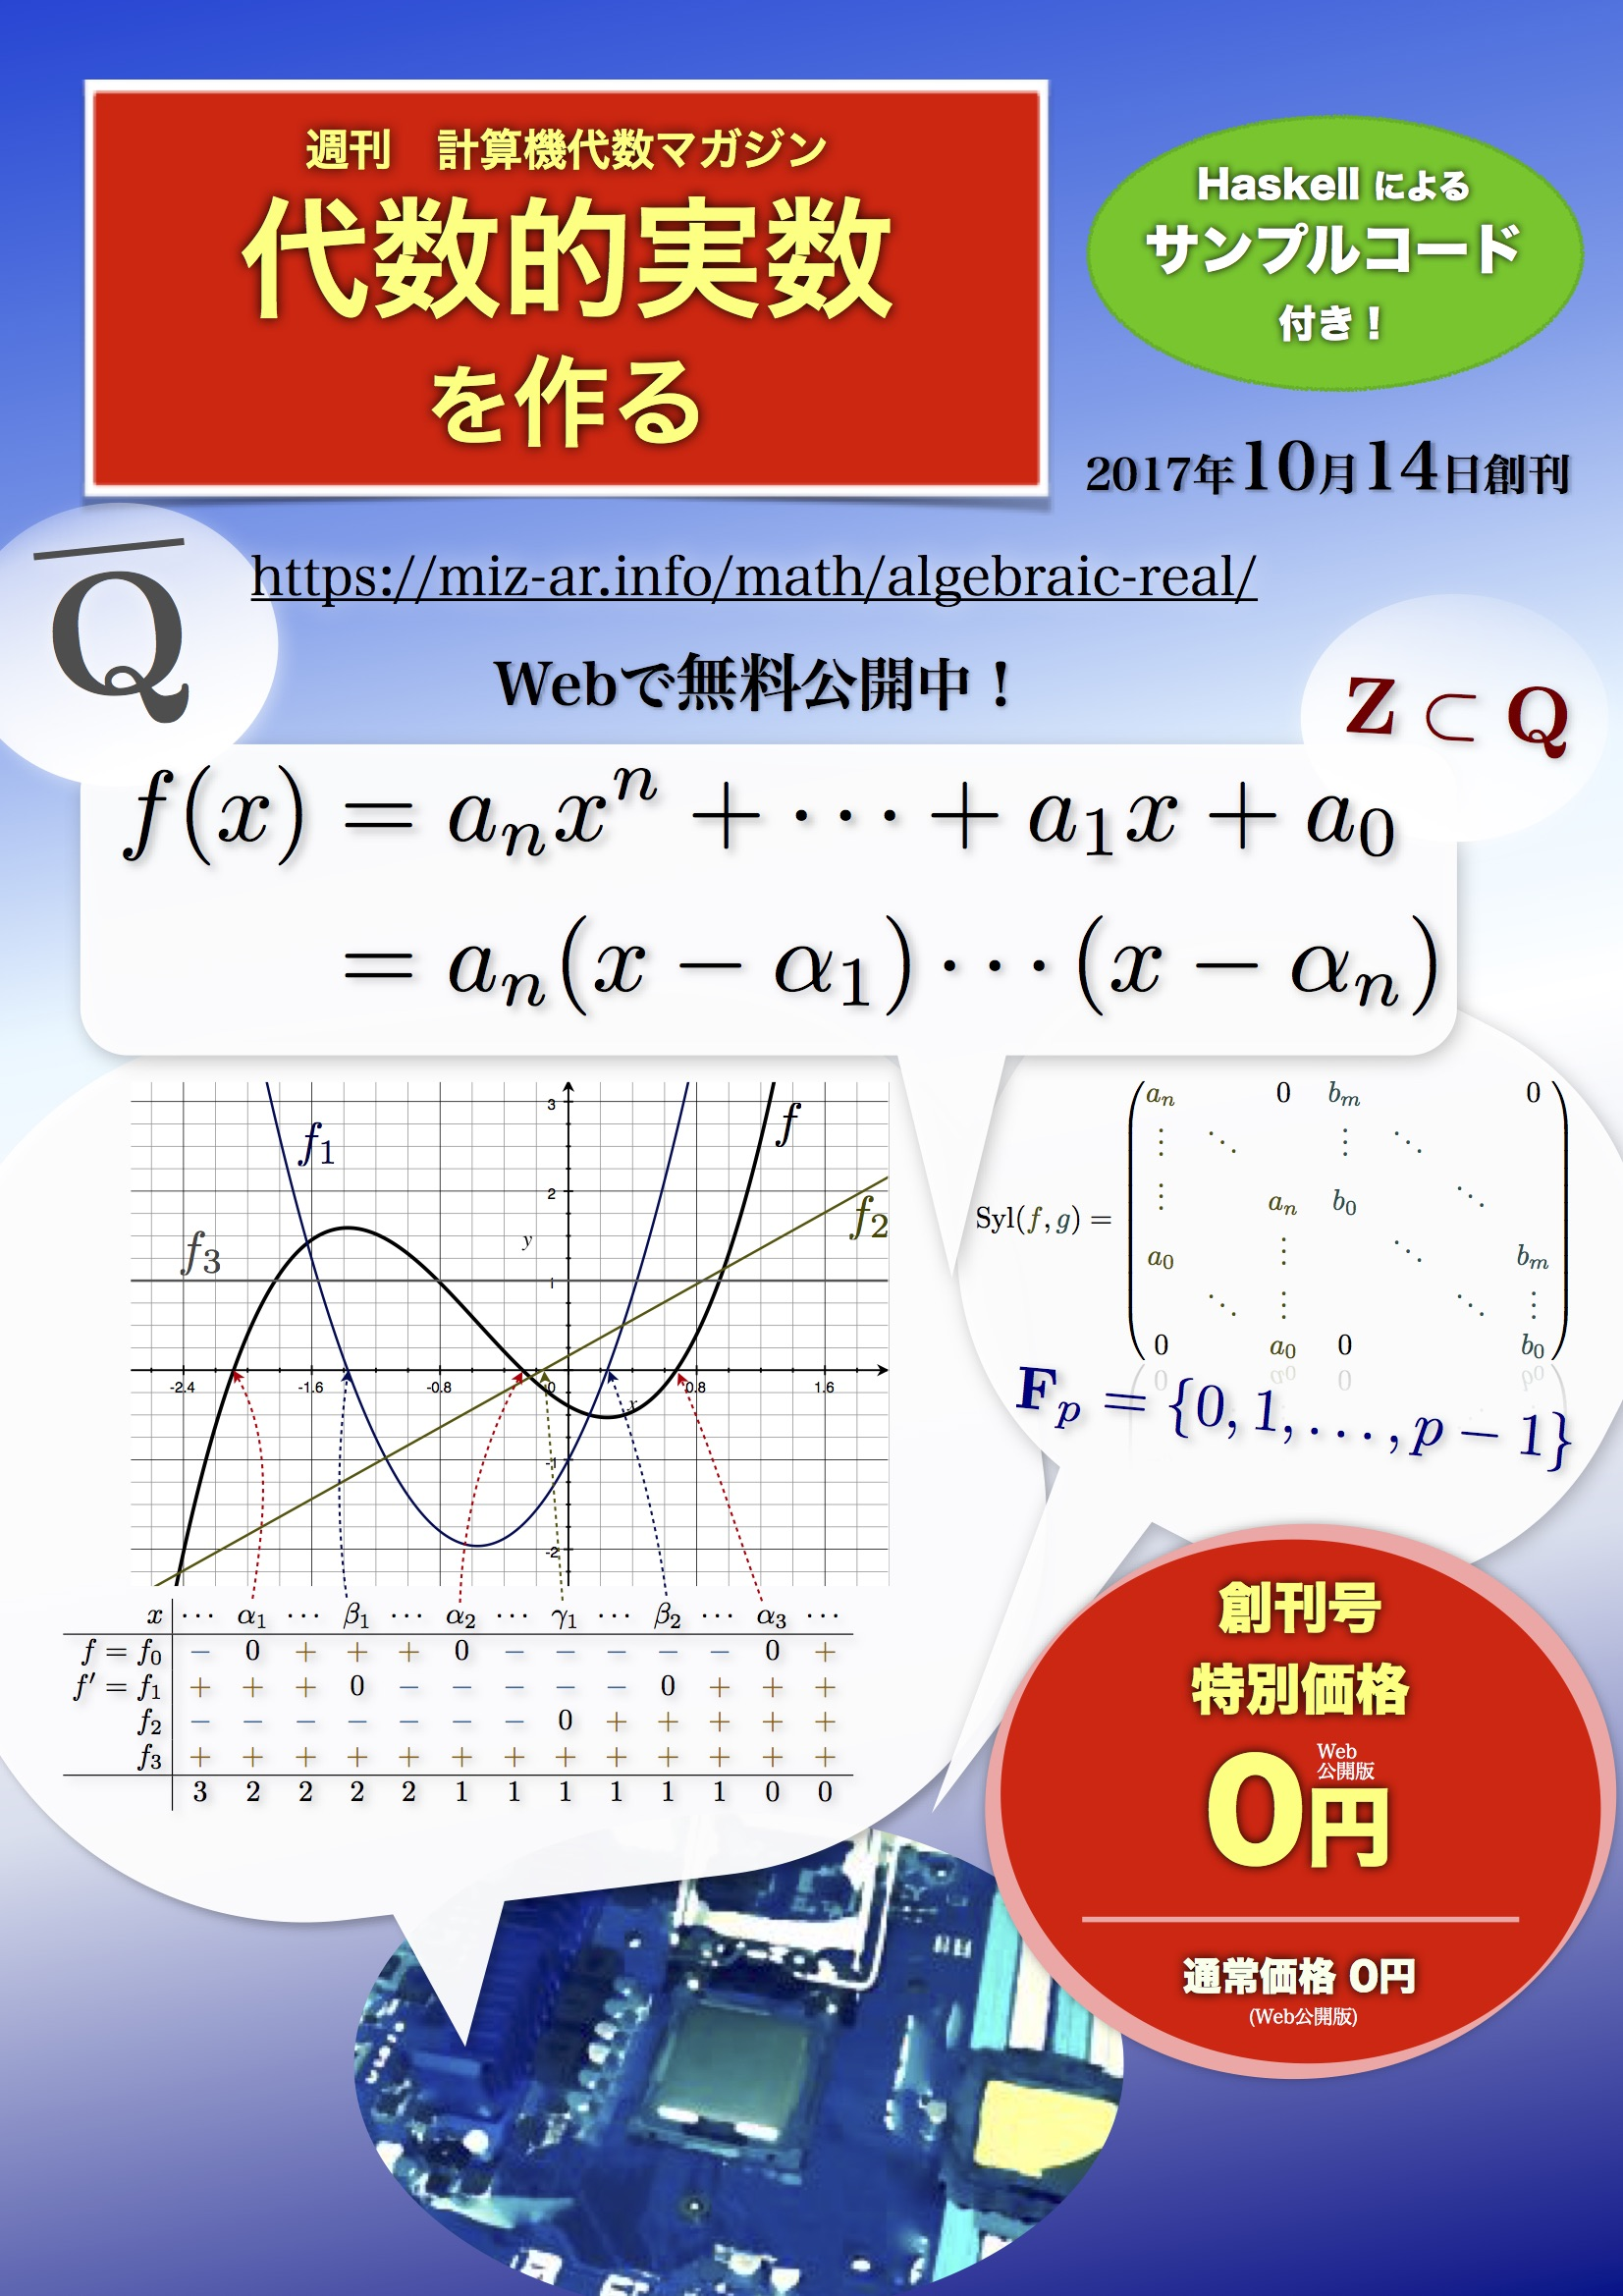
\includegraphics[height=0.96\textheight]{algreal.jpg}}
  \hspace{0.5em}
  \begin{minipage}{22em}
    「週刊 代数的実数を作る」 \newline
    \#4まで絶賛公開中! \newline
    \url{https://miz-ar.info/math/algebraic-real/}
  \end{minipage}
\end{frame}
\begin{frame}\frametitle{}
  \titlepage
\end{frame}
\begin{frame}\frametitle{目次}
  \tableofcontents
\end{frame}
\section{続・浮動小数点数の話}
\begin{frame}{丸め}
  浮動小数点数では、実数やその演算結果を正確に表せないことがある

  \begin{block}{例}
    1/10 は2進の有限桁で正確に表せない(循環小数になる)
  \end{block}

  \begin{block}{例}
    \(\sqrt{2}\), $e$, $\pi$ は正確に表せない(無理数なので)
  \end{block}
\end{frame}
\begin{frame}{丸め}
  そういう場合は「最も近い浮動小数点数」への\emph{丸め}を行う

  IEEE754では
  \begin{itemize}
  \item 四則演算(FMA含む)
  \item 平方根
  \end{itemize}
  が正しく丸められることを要請している。

  それ以外の数学関数(exp とか sin とか)は正しく丸められる保証はない!
\end{frame}
\begin{frame}{最近接丸め}
  \emph{最近接丸め}は最もポピュラーな丸め方向。
  「一番近い」浮動小数点数に丸める。

  ちょうど中間の場合は、最下位ビットが0になる方を選択する。
  \begin{block}{例}
    \(1+2^{-53}\) に一番近い倍精度浮動小数点数は $1$ と $1+2^{-52}$ の2つ。
    最下位ビットが0の方を選択する:
    \[1+2^{-53}\leadsto 1\]
  \end{block}
\end{frame}
\begin{frame}{方向付き丸め}
  それ以外の丸め方向
  \begin{itemize}
  \item 正の無限大方向
  \item 負の無限大方向
  \item ゼロ方向
  \end{itemize}
  これらは\emph{区間演算}で重要
\end{frame}
\begin{comment}
\begin{frame}{用語}
  \begin{block}{Machine epsilon}
    \begin{itemize}
    \item 1と、その次に大きい浮動小数点数の差
    \item 倍精度だと \(2^{-52}\approx 2\times10^{-16}\)
    \item 計算結果の有効数字、相対誤差の目安となる
    \end{itemize}
  \end{block}

  \begin{block}{ULP (unit in the last place)}
    \begin{itemize}
    \item 与えられた実数 \(x\) に対して、 \(x\) の周辺における浮動小数点数の間隔
    \item (\(x\) が浮動小数点数で表せない場合は) \(x\) の次に大きい浮動小数点数と \(x\) の次に小さい浮動小数点数の差
    \item 例文:最近接丸めの場合、演算結果の誤差は 0.5ulp 以内である。
    \end{itemize}
  \end{block}
\end{frame}
\end{comment}
\begin{frame}{実際のプログラミング言語では}
  \begin{itemize}
  \item C言語は実用的な言語なので、浮動小数点数の丸め方向を制御できる
    \begin{itemize}
    \item \texttt{<fenv.h> fesetround/fegetround} 関数
    \item \texttt{\#pragma STDC FENV\_ACCESS ON} で最適化を抑制
    \end{itemize}
  \item Juliaも実用的
  \end{itemize}
\end{frame}
\section{区間演算の話}
\begin{frame}{数値計算の信頼性}
  浮動小数点数を使って計算した結果は信頼できない?
\end{frame}
\begin{frame}{数値計算の信頼性}
  \emph{区間演算}を使うと、数値計算の結果がどれだけ信頼できるのか(誤差の範囲)がわかる!
\end{frame}
\begin{frame}{区間演算}
  取りうる値の上界と下界の組を使って演算する

  \begin{align*}
    [\lb{a},\ub{a}]+[\lb{b},\ub{b}]&=[\lb{a}+\lb{b},\ub{a}+\ub{b}], \\
    [\lb{a},\ub{a}]-[\lb{b},\ub{b}]&=[\lb{a}+\ub{b},\ub{a}-\lb{b}], \\
    [\lb{a},\ub{a}]\cdot[\lb{b},\ub{b}]&=[\min\{\lb{a}\lb{b},\lb{a}\ub{b},\ub{a}\lb{b},\ub{a}\ub{b}\},\max\{\lb{a}\lb{b},\lb{a}\ub{b},\ub{a}\lb{b},\ub{a}\ub{b}\}].
  \end{align*}
  区間に0を含まない場合は割り算もできる

  浮動小数点数を使って実装する場合は、各演算において方向付き丸めを行う

  (このほかに、区間の中心と半径を使う方式もある)
\end{frame}
\begin{frame}{アルゴリズムへの適用}
  各種アルゴリズムを区間演算に置き換える

  \begin{block}{例}
    \emph{区間ガウス消去法} (Interval Gaussian elimination)
  \end{block}

  頑張れば、普通の数値計算の数倍程度の実行時間で済む
\end{frame}
\begin{frame}{欠点}
  \begin{itemize}
  \item 演算を繰り返すと値の範囲が広がってしまう
  \item 「演算結果は $\pm$100万の範囲にあります(ドヤァ」と言われても嬉しくない!
  \item ゼロ除算が起きやすくなる
  \end{itemize}

  工夫が必要。\emph{平均値形式}など
\end{frame}
\end{document}
